\section*{第二章~~暗物质存在的观测证据}
\setcounter{section}{2} \setcounter{subsection}{0}
\setcounter{table}{0} \setcounter{figure}{0} \setcounter{equation}{0}
\addcontentsline{toc}{section}{第二章~~暗物质存在的观测证据}

尽管暗物质无法通过电磁波直接观测,但多种独立的天文观测一致地表明,在宇宙的各个尺度上都存在着某种“不可见”的质量成分。以下三类观测证据构成了暗物质存在的最直接、最重要的实证基础。

\subsection{星系旋转曲线(Galaxy Rotation Curves)}

星系旋转曲线是指星系中恒星和气体的圆周速度随其距离星系中心变化的曲线。它反映了星系内部质量分布对恒星和气体运动的影响。

星系旋转曲线有两种测量方法。光谱学方法:通过测量星系中恒星和气体的光谱线,可以确定它们的多普勒位移,从而计算出它们的径向速度。结合星系的几何结构,可以推导出恒星和气体的圆周速度;射电天文学方法:利用射电望远镜观测星系中的中性氢(HI)气体发射的21厘米线,可以确定气体的运动速度。这种方法特别适用于观测星系的外边缘区域,因为这些区域的恒星密度较低,光学观测较为困难。

1914年,Wolf和Slipher发现仙女座星系(M31)的光谱线在星系主轴方向上倾斜,在短轴方向上则为直线,从而得出仙女座星系在旋转的结论。

1939年,Horace Babcock在他的博士论文中,测量了仙女座星系的旋转曲线,发现其在大半径处的圆周速度非常高,暗示星系外侧存在大量质量。

自1970年代起,Vera Rubin 和 Kent Ford 等人对多个螺旋星系的旋转曲线进行观测,发现实际数据与经典预言严重不符:在远离星系中心的区域,恒星的轨道速度并未下降,而是趋于平坦。这意味着在星系外围区域仍存在大量未被观测到的质量,其引力足以维持恒星的高速旋转。

\begin{figure}[!htbp]
    \centering    
    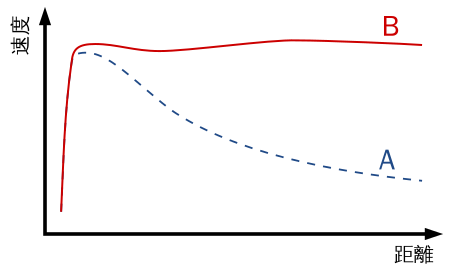
\includegraphics[height=3cm]{Img/2-1.png}
    \caption{星系旋转曲线:预测的(A)和观测的(B)。 }
    \label{2-1}
\end{figure}

根据牛顿引力定律,如果星系的质量主要集中在可见的恒星和气体中,那么随着到星系中心距离的增加,恒星和气体的圆周运动速度应该逐渐下降。然而,观测到的星系旋转曲线在大半径处保持平坦,这表明在星系的外围存在大量未被观测到的质量,这些质量无法用可见的恒星和气体来解释,从而为暗物质的存在提供了有力证据。

\subsection{引力透镜效应(Gravitational Lensing)}

根据广义相对论,质量分布可以导致时空弯曲,进而使背景天体发出的光线发生偏折,这一现象称为引力透镜效应。在天文学中,引力透镜被用作测量系统总质量的重要手段,尤其是在星系团尺度。

\begin{figure}[!htbp]
    \centering    
    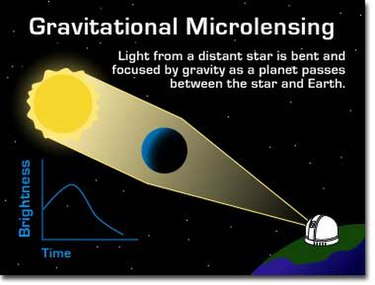
\includegraphics[height=5cm]{Img/2-2.jpg}
    \caption{引力透镜效应 }
    \label{2-2}
\end{figure}

通过对多个星系团的引力透镜效应进行分析,可以发现引力作用远远超过可见物质所能提供的水平。例如,在著名的子弹星系团(Bullet Cluster)中,两个星系团发生高速碰撞:X射线观测显示热气体集中在中心,而引力透镜揭示的质量分布却偏移至两个星系团的外围部分。换言之,引力“重心”不在可见质量重心所在的位置。这一现象被广泛认为是“可见物质无法解释全部引力作用”的直接证据。引入“不可见但有质量”的暗物质成分能够自然地解释质量分布与光偏折之间的关系。此外,弱引力透镜在大范围宇宙尺度上也支持类似结论:通过引力透镜效应观测得到的总质量普遍高于可见质量之和。

\subsection{宇宙微波背景(Cosmic Microwave Background)}

1965年,Arno Penzias和Robert Wilson在贝尔实验室进行射电天文学研究时,意外地发现了一种来自宇宙各个方向的均匀背景辐射。这种辐射的温度约为2.7 K,频率分布符合黑体辐射的谱线。这一发现被确认为宇宙微波背景辐射(Cosmic Microwave Background, CMB),为大爆炸理论提供了直接的观测证据。

宇宙微波背景辐射是大爆炸残留下的热辐射,携带着早期宇宙密度扰动的信息。通过对CMB各个多极谱峰的位置与高度进行精密测量(如 WMAP、Planck 计划),研究者可以推断宇宙的基本成分比例。

\begin{figure}[!htbp]
    \centering    
    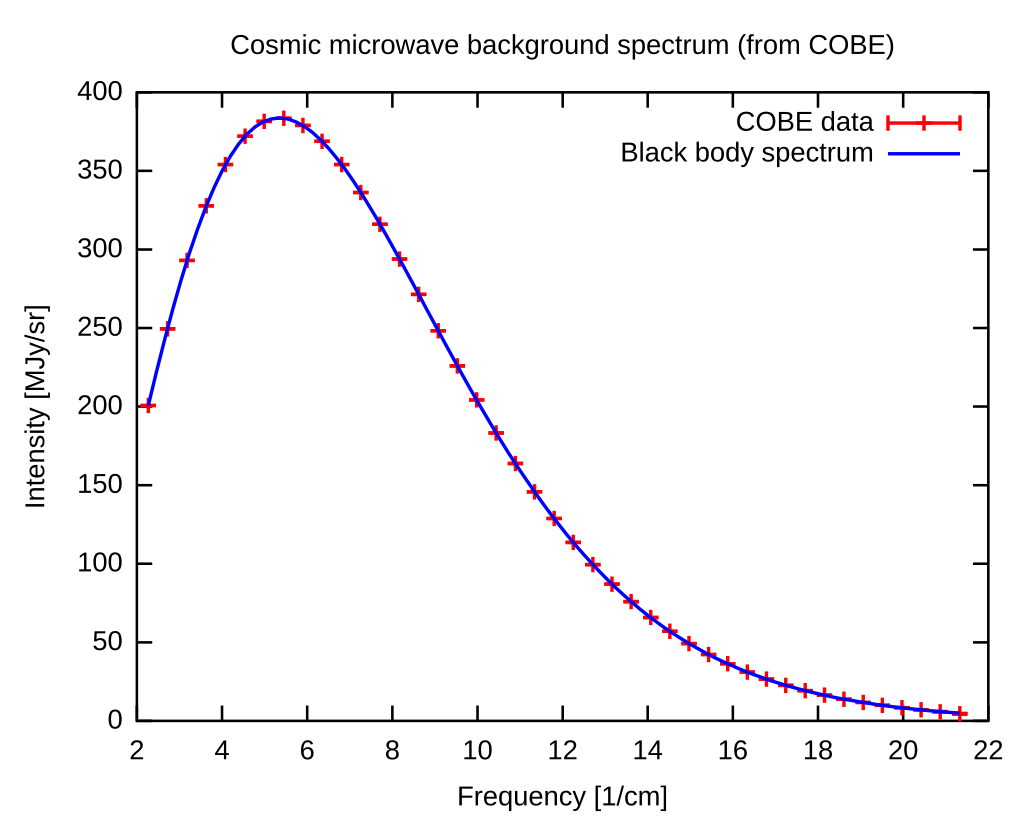
\includegraphics[height=5cm]{Img/2-3.png}
    \caption{由FIRAS仪器对COBE观测的宇宙微波背景辐射光谱 }
    \label{2-3}
\end{figure}

暗物质的存在会改变CMB功率谱的形状。通过分析CMB功率谱,可以推断出宇宙的总物质密度、暗物质密度和可见物质密度等宇宙学参数。这些测量结果与星系旋转曲线、引力透镜效应等其他观测结果一致,为暗物质的存在提供了有力证据。

CMB的温度分布存在微小的涨落,这些涨落反映了宇宙早期的密度不均匀性。通过分析CMB的温度涨落,可以推测宇宙的总物质密度、暗物质密度和可见物质密度。CMB的观测结果表明,暗物质约占总物质密度的85\%,而可见物质仅占15\%左右。

\newpage